\section{Background}
\subsection{A Closer Look At The Problem}
We can consider a current scientific application in order to better understand the problem Optika is trying to solve. 
Currently, the program Tramonto has a large input file filled with complex, non-intuitive inputs. Figure
\ref{tramontoInputFigure} is just small section of this input file.
\begin{figure}
  \centering
  {\footnotesize
  \begin{Verbatim}
************* DIMENSION PARAMETERS ********************************************
@ -1. -1. -1. -1. 10. 	Length_ref Density_ref Temp Dielec_ref VEXT_MAX 
************* MESH PARAMETERS *************************************************
@ 3 	Ndim 
@ 3. 2. 2. 	Size_x(idim): idim=0,Ndim-1 
@ 0.25 0.25 0.25 	Esize_x(idim): idim=0,Ndim-1 
@ -1 2 	Type_bc(x0,: left, right) 
(-1=IN_WALL, 0=IN_BULK, 1=PERIODIC, 2=REFLECT, 3=LAST_NODE) 
@ 1 1 	Type_bc(x1,: down, up) 
@ 1 1 	Type_bc(x2,: back, front) 
  \end{Verbatim}
  }
  \caption[Tramonto Input]{A portion of the complex input file used by Tramonto}
  \label{tramontoInputFigure}
\end{figure}

This input file is hard to read and non-intuitive, not to mention it could 
easily intimidate a new user. In fact, Tramonto's current input system is so complicated
that it is recommended most users simply take provided sample input files and just
modify them for their needs. Optika aims to solve this problem of complex input methods by allowing developers
like those of Tramonto to specify their required inputs, and let Optika handle the actual retrieval of
input values. The actual method of gathering input is completely abstracted away from the application developer.

\subsection{Why Not Something Else?}
Instead of relying on current GUI solutions to solve the above problem, Optika was created in order to address
a number of constraints.

\subsubsection{Something Simple}
Current GUI frameworks like Qt (on which Optika is based), GTK+, and Cocao are incredibly robust. But
because of this, they are also large and complicated. When looking for a solution to the 
scientific application interface problem, something simple is required. Otherwise, developers will be hesitant to use it.

\subsubsection{Cross-Platform}
Having a better user interface can lead to having a wider user base. But when adding the functionality
of a GUI to an application, a developer does not want to accidentally exclude some users by
using a technology that will not work on their users' platform of choice. Cocao, for example, only works on
Mac OSX systems. By using the Qt Framework as its underpinnings, Optika is able to work on a wide variety of
platforms.

\subsubsection{Trilinos Integration}
Optika was developed as part of the Trilinos project. Trilinos is a set of C++ libraries
used extensively throughout the scientific community. Since Optika is part of Trilinos,
it was desirable to have tight integration with constructs that were already in place inside
of Trilinos (namely the ParameterList class). By creating our own GUI solution, Optika allows 
users already familiar with the Trilinos framework to take advantage of the capabilities 
Optika has to offer.

\section{Optika Overview}
\subsection{GUI Fundamentals}
An Optika based GUI is laid out in a hierarchical fashion as shown in Figure \ref{paramlistFigure}.
This hierarchy is made up of parameters and parameter lists. A parameter can be thought of simply as single key-value input pair for
a program. A parameter list is a collection of parameters and other parameter lists. When a parameter list
is part of another parameter list, it is called a sublist. Optika then uses these parameter lists to dynamically
generate a GUI which is used to obtain input from the user.
\begin{figure}
  \centering
  \begin{picture}(50,150)(0,0)
    \put(10,0){\line(0,1){145}}
    \put(0,150){${Parameter List}$}
    \put(10,130){\line(1,0){15}}
    \put(28,127){$Parameter$}
    \put(10,110){\line(1,0){15}}
    \put(28,107){$Parameter$}
    \put(10,90){\line(1,0){15}}
    \put(28,87){$Parameter$}
    \put(10,70){\line(1,0){15}}
    \put(28,67){$Parameter List$}
    \put(38,0){\line(0,1){62}}
    \put(38,47){\line(1,0){15}}
    \put(56,44){$Parameter$}
    \put(38,22){\line(1,0){15}}
    \put(56,24){$Parameter$}
  \end{picture}
  \caption[GUI Layout]{The hierarchical layout of an Optika GUI}
  \label{paramlistFigure}
\end{figure}

Parameters in Optika are typed. Parameters can be any one of the following types:
	\begin{itemize}
		\item int and short
		\item float and double
		\item string
		\item boolean
		\item arrays of int, short, double, and string
		\item 2D arrays of int, short, double, and string
	\end{itemize}
When editing a parameter in Optika, different ``widgets'' are used to change the parameters value. A widget is 
a graphical construct used for obtaining input from the user. For number types, a spin box (Figure~\ref{spinboxfig}) is used to obtain input. 
If the valid values for a string type are specified (something that will be discussed later), a combo box (Figure~\ref{comboboxfig}) is used to obtain
input for that parameter.
Otherwise a line edit (Figure~\ref{lineeditfig}) is used to edit a string parameter. For booleans, a combo box (Figure~\ref{comboboxfig}) 
is also used. For arrays, a pop-up box containing numerous input widgets is used. The input widgets' type is determined by the
array type (e.g. for numerical, types a series of spinboxes is used; for string types, comboxes or lineedits are used, etc.). 

\begin{figure}
	\centering
	\subfigure[A Spin Box]{
		\label{spinboxfig}
		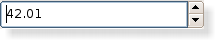
\includegraphics[scale=0.5]{graphics/spinbox}
	}
	\subfigure[A Combo Box]{
		\label{comboboxfig}
		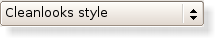
\includegraphics[scale=0.5]{graphics/combobox}
	}
	\subfigure[A Line Edit]{
		\label{lineeditfig}
		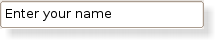
\includegraphics[scale=0.5]{graphics/lineedit}
	}
	\caption{Some of the various widgets used for editing data in Optika~\cite{QtGallery}}
	\label{editingWidgets}
\end{figure}

When all of these components are put together, the result is a basic Optika GUI looks something like Figure~\ref{basicexample}.
When the user clicks on a particular value, one of the above widgets pops up allowing them to edit the value.
Once the user is finished entering input, the user clicks the action button (labeled ``Submit'' in Figure~\ref{basicexample}).
The GUI then closes and the ParameterList used to help create the GUI now contains the input specified by the user.

\begin{figure}
\centering
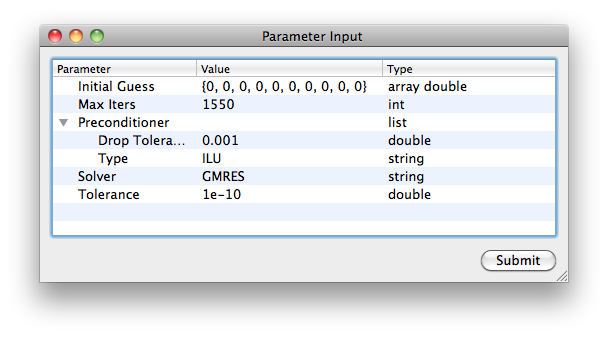
\includegraphics[scale=0.5]{graphics/basic_example}
\caption[Basic GUI]{A basic Optika GUI}
\label{basicexample}
\end{figure} 

\subsection{Underlying Technologies}
Optika is one of many packages in the Trilinos project~\cite{trilinos} which is developed primarily at Sandia National Labs. At its core, 
the Trilinos project is a collection of various
libraries for aiding developers of scientific applications. Trilinos is best known for its extensive collection of equation solvers,
but also provides a wealth of other tools that support general high performance computing. Each package in the Trilinos project provides
its own set of unique capabilities. Optika is the Trilinos GUI package.

In order to provide GUI functionality, Optika relies on the Qt Framework~\cite{Qt}. 
Qt was chosen as Optika's backing GUI framework for several reasons:
	\begin{itemize}
		\item It is cross-platform, allowing Optika to be used in many different computing environments.
		\item It is mature and has a comprehensive set of development tools. 
		\item It has a rich feature-set, permitting Optika to grow in its capabilities if necessary.
		\item It has been used by Sandia in the past.
		\item The Optika lead developer was familiar with it.
	\end{itemize}

In order to configure and build Optika, the CMake~\cite{cmake} build system is used. This is the build system
used by Trilinos as a whole, so it makes perfect sense for Optika to use it as well. In addition, CMake
has support for the necessary special building tools required by Qt.

\section{Basic Optika Usage}
At the core of Optika is the ParameterList class from the Teuchos package~\cite{TeuchosPackage}, another part
of the Trilinos project. ParameterLists can be constructed either from within C++ source code or using XML.
In this paper, we will first start off with a basic example using C++ source code. However, once we start
talking about more complex features, we will switch over to XML.
\subsection{Utilizing C++ to Create A GUI}
Looking at the sample Tramonto input file above, we can see how Optika could be used to create a better user interface.
While examining the example input file section, we see it deals with ``Dimension Control Parameters.'' These are a group of parameters 
used to define what kind of dimensions are going to be used in the rest of the input file. Figure~\ref{basicTramonto} shows how we would create
a GUI for these inputs.

\begin{figure}
\centering
{\footnotesize
\VerbatimInput{basicTramonto/main.cpp}
}
\caption{Basic Tramonto Example}
\label{basicTramonto}
\end{figure}
We start by including the Optika\_GUI.hpp file. This include file allows us to use most of Optika's basic functionality.
Once in the main function we import several classes and functions into the namespace. We then create two
ParameterList RCPs~\cite{RCP}. Using the sublist function, the second 
ParameterList is defined as a sublist of the first. We provide the lists with the names ``Tramonto'' and
``Dimension Control Parameters.'' The next several lines are calls to the ``set'' function. Each call
adds a Parameter to the ParameterList along with assigning it a default value and a documentation string (the 
documentation string is optional but highly encouraged). We then make
the all important call to the ``getInput'' function. This takes the list of parameters we have created and dynamically
generates a GUI which is then used to obtain input from the user. The end result is Figure~\ref{BasicTramontoScreenshot}.
\begin{figure}
\centering
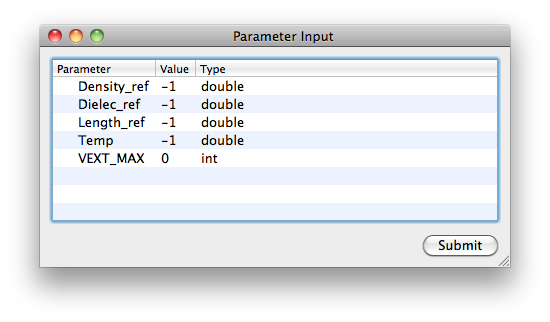
\includegraphics[scale=0.5]{graphics/BasicTramontoScreenshot}
\caption{The final product of the code in Figure~\ref{basicTramonto}}
\label{BasicTramontoScreenshot}
\end{figure}

\subsection{Utilizing XML to Create a GUI}
Using XML to declare input parameters has a number of advantages over declaring inputs in C++ source code.
\begin{itemize}
  \item XML is a lot cleaner than the corresponding C++. The source code approach can get unruly, especially
  when some of the more advanced features of Optika are used.
  \item As an extension of being cleaner, using XML makes maintaining a user interface much simpler.
  \item When using XML, there is no need to recompile the entire program every time a small change is made to the GUI.
\end{itemize}
If we redo the example we made in the previous section, but using XML, we end up with the C++ code and XML code found in
Figure~\ref{basicXMLC++} and Figure~\ref{basicXMLXML} respectively. The XML code is rather straight-forward. As in the C++ code, we specify 
the name of the parameter, its default value, and a documentation string (the documentation XML attribute is optional, just like when using 
C++). When using XML, we need to explicitly specify the type
of the parameter since this cannot always be inferred from XML. Creating a ParameterList hierarchy is also arguable easier
in XML. ParameterLists just simply need to be nested in one another.

Once the XML file describing the input parameters has been created, the GUI is created by using a slightly different
call to the getInput function. In this case, the getInput function is passed the name of the XML file and an RCP pointing
to the ParameterList into which user input should be stored.
\begin{figure}
{\footnotesize
\centering
\VerbatimInput{basicXMLTramonto/main.cpp}
}
\caption{The supporting C++ source code needed to utilize the XML in Figure~\ref{basicXMLXML}}
\label{basicXMLC++}
\end{figure}
\begin{figure}
{\footnotesize
\centering
\VerbatimInput{basicXMLTramonto/inputs.xml}
}
\caption{The XML that can be used to generate the same GUI as in Figure~\ref{basicTramonto}}
\label{basicXMLXML}
\end{figure}

\section{Validators}
Often input parameters only have a certain set of valid values. Through the use of validators Optika allows application
developers to express these parameter constraints. When a validator is placed on a parameter, the generated GUI will
not accept invalid parameter values. Like parameter lists, validators were also already part of the Teuchos package
before Optika was built. However, the existing set of validators was sparse. Optika took the validator constructs that
were already in place and built on them, resulting in the construction of several new types of validators detailed below.
These new validators were then placed in the Teuchos package.

Validators are declared in a special section of the XML file. A special <Validators> tag is declared as a direct child
of the root <ParameterList> tag. In this <Validators> tag all validators are declared. Each validator must specify at
least its type and an Id using the <Validator> tag. This Id can then be used anywhere in the rest of the XML file. 
To apply the validator to a parameter, simply add the validatorId XML attribute to the <Parameter> tag. The same validator 
can be used on multiple parameters.

\subsection{Enhanced Number Validators}
Perhaps one of the most important validators is the Enhanced Number Validator. It allows the application developer
to specify minimum and maximum values for a numerical parameter (both inclusive). It also allows the developer to specify the
``step'' of a numerical parameter. The step of a numerical parameter is the amount by which the parameter's value
will be increased or decreased when the user clicks the up and down arrows on the spinbox being used to edit
the parameter's value. For non-integer numerical parameters, the Enhanced Number Validator also allows the
developer to declare with what precision the parameter's value should be displayed to the user.

The XML in Figure~\ref{EnhancedNumberValidatorXML} shows an example of using an Enhanced Number Validator
to validate a parameter of type double. In the example, we set the minimum acceptable value to be 0 and the 
maximum to be 10. The step is set to .5 so that the parameters value will change by .5 when the user clicks
up or down in the spinbox being used to edit the parameter. We also set the precision to two decimal places.
The validator is given the Id of 1 and applied thusly to the ``Double Parameter'' parameter using the validatorId
XML attribute. Notice how the ``type'' XML attribute of the validator is set to ``EnhancedNumberValidator(double)''. If we 
were validating a parameter of type int, this XML attribute would be set to ``EnhancedNumberValidator(int)'', 
for a float it would be ``EnhancedNumberValidator(float)'', etc. These types must match up, otherwise an error will
occur.

With the exception of the validatorId XML attribute, all validator XML attribute demonstrated in Figure~\ref{EnhancedNumberValidatorXML}
are optional for an Enhanced Number Validator. For example, a developer could only specify a minimum value of 0 to restrict all 
values of a parameter to positive values since no maximum was specified.
Appropriate defaults will be selected for step and precision if the developer chooses not to specify them.
\begin{figure}
\centering
{\footnotesize
\begin{Verbatim}
<ParameterList>
  <Parameter name="Double Parameter" value="1.0" type="double" 
    docString="A double parameter" validatorId="1" />
    ...Other Parameters ....
  <Validators>
    <Validator type="EnhancedNumberValidator(double)" 
      min="0" max="10" step=".5" precision="2" validatorId="1"/>
  </Validators>
</ParameterList>
\end{Verbatim}
}
\caption{Example usage of an Enhanced Number Validator}
\label{EnhancedNumberValidatorXML}
\end{figure}

\subsection{String Validators}
String Validators are a simple yet powerful tool for restrict string input. String input can be a nice alternative to
using some standard set of integer values to represent various settings for a parameter. The problem is a simple wrong 
keystroke can cause big problems. By using a String Validator, an application developer can ensure that a user 
only selects a string value that is appropriate for a given parameter. 
String Validators may only be used on parameters of type std::string, otherwise an error will occur.

Figure~\ref{StringValidatorXML} shows how to use a String Validator. Children <String> tags with a mandatory ``value'' XML attribute specify which values are 
valid.  In this example, ``Option 1'', ``Option 2'', and ``Option 3'' will be the only values the user can select from in the GUI.
\begin{figure}
\centering
{\footnotesize
\begin{Verbatim}
<ParameterList>
  <Parameter name="String Parameter" value="Option 1" type="string" 
    docString="A string parameter" validatorId="1" />
    ...Other Parameters ....
  <Validators>
    <Validator type="StringValidator" validatorId="1">
      <String value="Option 1"/> 
      <String value="Option 2"/> 
      <String value="Option 3"/> 
    </Validator>
  </Validators>
</ParameterList>
\end{Verbatim}
}
\caption{Example usage of a String Validator}
\label{StringValidatorXML}
\end{figure}

\subsection{Filename Validators}
Filename Validators allow application developers to designate a string parameter as a filename. When applied to a parameter,
any attempt to edit that parameter will result in the user being presented with a special file selector widget (Figure~\ref{fileSelectorWidget}). If the 
``fileMustExist'' XML attribute is set to true, the user will only be able select files that already exist. Otherwise, any file may be selected by the user.
Filename Validators can only be applied to parameters of type string. 

Figure~\ref{filenameValidatorXML} shows an example of how to use a Filename Validator. Here we use it to select a file to output the results
of our program. We set the ``fileMustExist'' XML attribute to false so that the user can select a file that does not already exist.
\begin{figure}
\centering
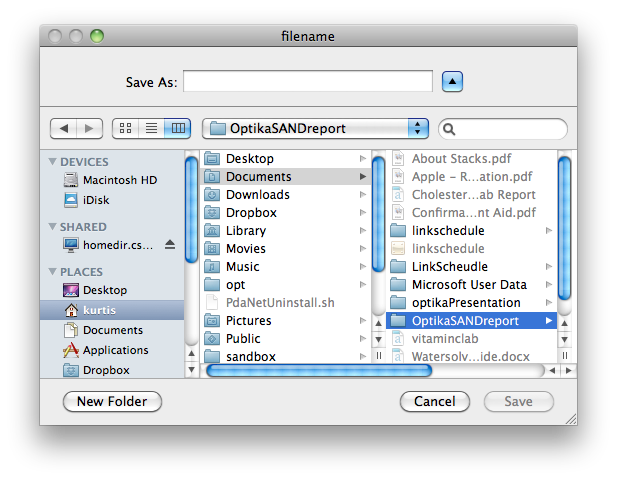
\includegraphics[scale=0.5]{graphics/fileWidget}
\caption{The file selector widget presented to the user when a Filename Validator is applied to a parameter}
\label{fileSelectorWidget}
\end{figure}

\begin{figure}
\centering
{\footnotesize
\begin{Verbatim}
<ParameterList>
  <Parameter name="Output File Name" value="" type="string" 
    docString="Name of the output file." validatorId="1" />
    ...Other Parameters ....
  <Validators>
    <Validator type="FilenameValidator" fileMustExist="false" 
      validatorId="1">
  </Validators>
</ParameterList>
\end{Verbatim}
}
\caption{Example usage of a Filename Validator}
\label{filenameValidatorXML}
\end{figure}

\subsection{Array Validators}
Array Validators allow any of the above described validators to be used on a array parameter. For example, we might want to use a
String Validator on an array of strings. To do this, we create and Array Validator with a ``prototype'' String Validator. The 
``prototype'' validator is just a term used to describe the validator the developer would like to be applied to each entry of an
array. Prototype validators can be specified in one of two ways. First, the developer can code the validator as child of the array validator
tag as in Figure~\ref{actualArrayValidatorXML}. In this case, the prototype validator does not need an Id. 
Second, the developer can simply specify another validator as array validator's  prototype by using the
``prototypeId'' XML attribute as in Figure~\ref{protoAttributeArrayXML}. This second option allows the developer to reuse the prototype validator in 
other instances.

When creating an Array Validator, the ``type'' XML attribute will include both the type of the prototype validator and the type of the array
parameter. For instance, if we were using a prototype Filename Validator on a string parameter, the value of our ``type'' XML attribute would
be ``ArrayValidator(FilenameValidator, string)''. It is crucial that all of these types match up. Otherwise, errors will occur.

\begin{figure}
\centering
{\footnotesize
\begin{Verbatim}
<ParameterList>
  <Parameter name="Options" value="{Option 1, Option 1, Option 1}" 
    type="Array(string)" docString="An array of options" 
    validatorId="1" />
    ...Other Parameters ....
  <Validators>
    <Validator type="ArrayValidator(StringValidator, string)" 
      validatorId="1">
      <Validator type="StringValidator">
        <String value="Option 1"/>
        <String value="Option 2"/>
        <String value="Option 3"/>
      </Validator>
    </Validator>
  </Validators>
</ParameterList>
\end{Verbatim}
}
\caption{Example usage of an Array Validator in which the prototype validator is declared as a child of the array validator}
\label{actualArrayValidatorXML}
\end{figure}

\begin{figure}
\centering
{\footnotesize
\begin{Verbatim}
<ParameterList>
  <Parameter name="Output File Name" value="{Option 1, Option 1}" 
    type="Array(string)" 
    docString="Name of output file." validatorId="1" />
    ...Other Parameters ....
  <Validators>
    <Validator type="ArrayValidator(StringValidator, string)" 
      validatorId="1" prototypeId="2"/>
    <Validator type="StringValidator" validatorId="2">
      <String value="Option 1"/>
      <String value="Option 2"/>
      <String value="Option 3"/>
    </Validator>
  </Validators>
</ParameterList>
\end{Verbatim}
}
\caption{Example usage of an Array Validator in which the prototype is specified using the prototypeId XML attribute}
\label{protoAttributeArrayXML}
\end{figure}

All the discussion above is also relevant for TwoDArrays. The only difference is instead of using an ArrayValidator, a TwoDArrayValidator is used. For
example, if a TwoDArray of arbitrary integer values needs to be restricted with an EnhancedNumberValidator, the XML in Figure~\ref{TwoDArrayValidator}
would be appropriate.
\begin{figure}
\centering
{\footnotesize
\begin{Verbatim}
<ParameterList>
  <Parameter name="Integer Values" value="2x2:{4,3,1,2}" 
    type="TwoDArray(int)" docString="A twod array of integers" 
    validatorId="1" />
    ...Other Parameters ....
  <Validators>
    <Validator type="TwoDArrayValidator(EnhancedNumberValidator(int), int)" 
      validatorId="1">
      <Validator 
        type="EnhancedNumberValidator(int)"
        min="0"
        max="10"
      />
      </Validator>
    </Validator>
  </Validators>
</ParameterList>
\end{Verbatim}
}
\caption{Example usage of a TwoDArrayValidator}
\label{TwoDArrayValidator}
\end{figure}


\section{Dependencies}
Dependencies are one of the most powerful tools provided by Optika~\footnote{Dependencies are actually found in the Teuchos package. However they were 
intentionally developed for use in Optika}.
They allow application developers to express common dependencies that occur between
parameters in their program. At their core, dependencies allow a developer to say ``based on the state of parameter A, parameter B should
behave in a certain way.'' In this case, we would say parameter A is the ``dependee'' parameter and parameter B is the ``dependent'' parameter.
All dependencies have at least one dependee and one dependent. When running the GUI, the algorithm for expressing dependencies is as follows:
\begin{enumerate}
	\item A parameter's value is changed by the end-user.
	\item The GUI queries the associated defined dependencies to see whether or not the parameter that changed has any dependents.
	\item If the parameter does have dependents, the GUI requests a list of all the dependencies in which the changed
	parameter is a dependee.
	\item For each dependency, the ``evaluate'' function is called. The dependency makes any necessary changes to the dependent parameter(s)
	and the GUI updates with the new data.
	\item If any dependents now have invalid values, focus is given to them and the user is requested to change their value to
	something more appropriate.
\end{enumerate}

Like validators, dependencies are declared in XML using the <Dependencies> tag. This tag must be a direct child
of the root <ParameterList> tag. Inside the <Dependencies> tag each dependency is declared using the <Dependency> tag. Within the
<Dependency> tag the XML attribute ``type'' is required in order to define the type of the dependency. Each <Dependency> must have at least
one <Dependee> child tag and one <Dependent> child tag. Each of these tags must have an XML attribute called ``parameterId'' which identifies
their associated parameter. A dependency must have an arbitrary number of dependents.

\subsection{Visual Dependencies}
Visual Dependencies allow the application developer to show and hide parameters based on other parameters' values. This is useful in situations
when a parameter takes on a particular value, and as a result, another parameter is no longer relevant. By hiding this now irrelevant parameter from the user the
application developer can hopefully avoid some confusion on the user's part. If we were to write these dependencies as a sentence, they would say: ``Based on
the value of the dependee parameter show or hide the dependent parameter(s)''.

Visual Dependencies have an extra boolean XML attribute that can be put in the <Dependency> tag called ``showIf''. Which ever dependee is being tested to 
determine the dependents visibility, showIf can negate it by being set to false. So if a visual dependency is set to only show a dependent when the
dependee has a particular value, setting showIf to false will cause the dependent to be visible only when the dependee \emph{does not} have a particular
value. If the showIf attribute is not present, it is assumed to be true. With Visual Dependencies, dependents can also be parameter lists in addition to regular
parameter dependents.

\subsubsection{String Visual Dependencies}
String Visual Dependencies allow an application developer to base whether or not a parameter is visible on the particular string value of another
parameter. For instance, we might say if the ``Favorite Food'' parameter  is equal to the value ``Cheddar Cheese'' or ``Swiss Cheese'' then show parameter ``Cheese Rating''. 
Otherwise, do not show parameter ``Cheese Rating''. Figure~\ref{StringVisXML} demonstrates how we would express this in XML. The 
``Cheese Rating'' parameter will only be shown when ''Favorite Food'' is set to ``Cheddar Cheese'' or ``Swiss Cheese''. String Visual dependencies must have a single 
dependee of type string. 
\begin{figure}
\centering
{\footnotesize
\begin{Verbatim}
<ParameterList>
  <Parameter name="Favorite Food" type="string" value="pasta"
    id="1" docString="Your favorite food."/>
  <Parameter name="Cheese rating" type="int" value="5"
    docString="A rating of cheese" id="2"
    ...Other Parameters ....
  <Dependencies>

    <Dependency showIf="true" type="StringVisualDependency">
      <Dependee parameterId="1"/>
      <Dependent parameterId="2"/>
      <StringValues>
        <String value="Swiss Cheese"/>
        <String value="Cheddar Cheese"/>
      </StringValues>
    </Dependency>

  </Dependencies>
</ParameterList>
\end{Verbatim}
}
\caption{Example usage of a String Visual Dependency}
\label{StringVisXML}
\end{figure}

\subsubsection{Bool Visual Dependencies}
Bool Visual Dependencies allow the developer to base the visibility of a parameter on the boolean value of another parameter. For instance, we might say
if parameter A is set to true then we want to show parameter list B. Figure~\ref{BoolVisXML} shows how a developer would implement this in XML. The
``Special Parameters'' list will only be shown when ``Use special parameters'' is set to true. Bool Visual Dependencies must have a single dependee of type bool.
\begin{figure}
\centering
{\footnotesize
\begin{Verbatim}
<ParameterList>
  <Parameter name="Use special parameters" type="bool" value="true"
    id="1" docString="Whether or not to use special parameters"/>
  <ParameterList name="Special Parmeters" type="int" id="2"
    docString="special parameters only used in certain instances" 
    ...Special Parameters ....
  </ParameterList>
  <Dependencies>

    <Dependency showIf="true" type="BoolVisualDependency">
      <Dependee parameterId="1"/>
      <Dependent parameterId="2"/>
    </Dependency>

  </Dependencies>
</ParameterList>
\end{Verbatim}
}
\caption{Example usage of a Bool Visual Dependency}
\label{BoolVisXML}
\end{figure}

\subsubsection{Number Visual Dependencies}
Number Visual Dependencies allow the developer to base the visibility of a parameter on the numerical value of another parameter. In their simplest form,
Number Visual Dependencies simply check to see if the dependee's value is greater then or equal to zero. If the value is greater than or equal to zero, the
dependent(s) will be shown. Otherwise, the dependent(s) will be hidden.
Figure~\ref{NumberVisXML1} shows basic usage of a Number Visual Dependency. Unless the ``Temperature'' parameter is below zero degrees
Celsius, then we cannot have any ice cubes in the room. We do this by setting the ``showIf'' XML attribute to false so that ``Number of ice cubes'' only shows
when the ``Temperature'' parameter is below zero.
\begin{figure}
\centering
{\footnotesize
\begin{Verbatim}
<ParameterList>
  <Parameter name="Temperature" type="double" value="1" id="1" 
    docString="The temperature in the room in degrees celsius"/>
  <Parameter name="Number of ice cubes" type="int" value="1"
    id="2" docString="The number of ice cubes in the room"/>
  <Dependencies>

    <Dependency 
      showIf="false" 
      type="NumberVisualDependency(double)"
    >
      <Dependee parameterId="1"/>
      <Dependent parameterId="2"/>
    </Dependency>

  </Dependencies>
</ParameterList>
\end{Verbatim}
}
\caption{Example usage of a Number Visual Dependency}
\label{NumberVisXML1}
\end{figure}

Notice in Figure~\ref{NumberVisXML1} that like Enhanced Number Validators, the ``type'' XML attribute of a Number Visual Dependency has to include the type of the
parameter it is evaluating (in this case a double). Number Visual Dependencies may have only one dependee. The type of that dependee must match up with the
type specified in the ``type'' XML attribute used in the Number Visual Dependency tag.

Sometimes it is necessary to test a number typed parameter using criteria other than whether or not its current value is greater than or equal to zero.
This can be accomplished by using a <Function> tag. A <Function> tag instructs the dependency to run the value of the dependee through a function
first, and then test the result of that function to see if it is greater than or equal to zero. Consider the example in Figure~\ref{NumberVisXML1}, only this
time we will specify our temperature is in degrees Fahrenheit. In order to get the proper functionality, we will add a ``subtraction function'' to the dependency that will
subtract 32 from the value of the temperature parameter before it is tested against zero. Figure~\ref{NumberVisXML2} shows an example of this. We set the operand 
XML attribute to ``32'' and the type of the function to ``SubtractionFunction(double)''\footnote{For a complete list of available functions see Appendix~\ref{sec:funcs}}
 since we want to use a subtraction function on a parameter of type double.
\begin{figure}
\centering
{\footnotesize
\begin{Verbatim}
<ParameterList>
  <Parameter name="Temperature" type="double" value="33" id="1" 
    docString="The temperature in the room in degrees farenheit"/>
  <Parameter name="Number of ice cubes" type="int" value="1"
    id="2" docString="The number of ice cubes in the room"/>
  <Dependencies>

    <Dependency 
      showIf="false" 
      type="NumberVisualDependency(double)"
    >
      <Dependee parameterId="1"/>
      <Dependent parameterId="2"/>
      <Function operand="32" type="SubtractionFunction(double)"/> 
    </Dependency>

  </Dependencies>
</ParameterList>
\end{Verbatim}
}
\caption{Example usage of a Number Visual Dependency using a function}
\label{NumberVisXML2}
\end{figure}

\subsection{Validator Dependencies}
A Validator Dependency is a dependency in which the validator that is in use on the dependee is dependent upon the value of the dependee. Both the type of
the dependee and the dependent will vary with each type of Validator Dependency and parameter type of the dependent. Validator Dependencies will always have
one dependee. Also, dependent parameters in a Validator Dependency will never be a parameter list. A Validator Dependency can have an arbitrary number of 
dependents.

\subsubsection{String Validator Dependency}
A String Validator Dependency allows the application developer to change the validator used on a dependent based on the string value of the dependee
parameter. This is accomplished by mapping values the dependee might take on to corresponding validators. Also, a default validator may be specified.
This way, if the dependee takes on a value that has not been mapped to a validator, the default validator can be used. If the dependee takes on a value
that is not specified in the values to validator mappings and no default validator is specified, then the dependee(s) will have no validator(s).

A String Validator Dependency must comply with the following rules:
\begin{itemize}
\item The dependee must be of type string.
\item At least one validator to value mapping must be supplied.
\item All of the validators which have values mapped to them must be of the same type.
\item If specified, the default validator must be of the same type of validator used in the map.
\item The validators in the map and the default validator should be appropriate for the parameter type of the dependent(s).
\end{itemize}

Figure~\ref{StringValiDepXML} shows an example of how to use a String Validator Dependency. In this example we have two parameters, 
``Favorite Food Type''
and ``Favorite Food''. If ``Favorite Food Type'' is set to ``Cheese'' we want to restrict the values on ``Favorite Food'' to only values that are names
of cheese. But if ``Favorite Food Type'' is set to ``Chips'', we want to restrict the ``Favorite Food'' values to names of chips. Note that if the user
sets the value of ``Favorite Food Type'' to something else other than ``Cheese'' or ``Chips'', there will be no validator on ``Favorite Food''. This can
be remedied by either providing the String Validator Dependency with a default validator or by adding a validator to ``Favorite Food Types'' which only
allows the user to enter in either ``Chips'' or ``Cheese''.
\begin{figure}
\centering
{\footnotesize
\begin{Verbatim}
<ParameterList>
  <Parameter name="Favorite Food Type" type="string" value="Cheese"
    id="1" docString="The type of your favorite food"/>
  <Parameter name="Favorite Food" type="string" value="American"
    id="2" docString="Your favorite food"/>
  ...Other Parameters...
  <Validators>
    <Validator type="StringValidator" validatorId="1">
      <String value="American"/>
      <String value="Swiss"/>
      <String value="Pepperjack"/>
    </Validator>
    <Validator type="StringValidator" validatorId="2">
      <String value="Lays"/>
      <String value="Ruffles"/>
      <String value="Pringles"/>
    </Validator>
  </Validators>
  <Dependencies>
    <Dependency type="StringValidatorDependency>
      <Dependee parameterId="1"/>
      <Dependent parameterId="2"/>
      <ValuesAndValidators>
        <Pair value="Cheese" validatorId="1"/>
        <Pair value="Chips" validatorId="2"/>
      </ValuesAndValidators>
    </Dependency>
  </Dependencies>
</ParameterList>
\end{Verbatim}
}
\caption{Example usage of a String Validator Dependency}
\label{StringValiDepXML}
\end{figure}

\subsubsection{Range Validator Dependency}
Range Validator Dependencies work very similarly to String Validator Dependencies in that they map validators to specific dependee values. However,
instead of mapping string values to validators, Range Validator Dependencies map ranges of numbers to validators. If the dependee's value falls within one of the 
mapped ranges, then that range's associated validator is applied to the dependent(s). A range is specified by defining its minimum (inclusive) and its maximum (exclusive) 
values. Also, like String Validator Dependencies, a default validator can be specified. If the dependees value does not fall with in one of the mapped ranges, the default 
validator is used. If the dependee takes on a value that is not specified in the values to validator mappings and no default validator is specified, then the 
dependee(s) will have no validator(s).

A Range Validator Dependency must conform to the following constraints:
\begin{itemize}
\item The dependee must be a number type.
\item At least one value to validator mapping must be supplied.
\item All of the validators used specified in the mapping must be of the same type.
\item If specified, the default validator must be of the same type as the validators specified in the map.
\item The validators specified in the map must be appropriate for the type of the dependent(s).
\item Ranges cannot intersect.
\end{itemize}

Figure~\ref{RangeValiDepXML} shows an example of a Range Validator Dependency. In it, we want to use different validators
on the ``Fondue Food'' if the ``Fondue Pot Temperature'' is different. If the temperature is greater than or equal to 80 or less than 120,
we only want the user to be able to select ``Cheese'' or ``Bread''. If it is greater than or equal to 120 but less than 180, we only want the
user to be able to pick ``Chicken'' or ``Beef''. We associated these ranges with their appropriate values in the <RangesAndValidators> tag by
using <Pair> tags for each range and validator. Notice that like Enhanced Number Validators and Number Visual Dependencies, the type of the dependee parameter is 
included in the ``type'' XML attribute of the dependency. In Figure~\ref{RangeValiDepXML} the dependee's type is double so the type of the dependency is 
``RangeValidatorDependency(double)''.
\begin{figure}
\centering
{\footnotesize
\begin{Verbatim}
<ParameterList>
  <Parameter name="Fondue Pot Temperature" type="double" value="100"
    id="1" docString="The number of dimensions being used"/>
  <Parameter name="Fondue Food" type="string" value="Cheese"
    id="2" docString="The food we're fonduing"/>
  <Validators>
    <Validator type="StringValidator" validatorId="1">
      <String value="Cheese"/>
      <String value="Bread"/>
    </Validator>
    <Validator type="StringValidator" validatorId="2">
      <String value="Chicken"/>
      <String value="Beef"/>
    </Validator>
  <Validators>
  <Dependencies>
    <Dependency type="RangeValidatorDependency(double)">
      <Dependee parameterId="1"/>
      <Dependent parameterId="2"/>
      <RangesAndValidators>
        <Pair min="80" max="120" validatorId="1"/>
        <Pair min="120" max="180" validatorId="2"/>
      </RangesAndValidators>
    </Dependency>
  </Dependencies>
</ParameterList>
\end{Verbatim}
}
\caption{Example usage of a Range Validator Dependency}
\label{RangeValiDepXML}
\end{figure}

\subsubsection{Bool Validator Dependency}
A Bool Validator Dependency allows the developer to apply one validator to the dependent(s) when the dependee is true, and another validator
to the dependent(s) when the dependee is false. You could also specify one validator to be applied when the dependee is true and no validator
to be applied when the dependee is false (or vice versa). The dependee of a Bool Validator Dependency must be of type bool. If both a ``true'' and
``false'' validator are specified, they must be of the same type. Also, the validator(s) specified must be appropriate for the dependent(s).

Figure~\ref{BoolValidDepXML} shows an example of a Bool Validator Dependency. In this example, we only want a validator to be placed on the
``Temperature'' parameter if ``Has Temperature Constraints'' is set to true. Therefore we set the trueValidatorId XML attribute to the id of the
validator we want to use and do not specify a validator to be used if the dependee is false.
\begin{figure}
\centering
{\footnotesize
\begin{Verbatim}
<ParameterList>
  <Parameter name="Has Temperature Constraints?" type="bool" 
    value="true" id="1" 
    docString="Whether or not to use temperature constraints."/>
  <Parameter name=" Temperature" type="double" value="0"
    id="2" docString="The temperature"/>
  <Validators>
    <Validator type="EnhancedNumberValidator(double)" validatorId="1"
      min="0" max="50"/>
  <Validators>
  <Dependencies>
    <Dependency 
      type="BoolValidatorDependency" 
      trueValidatorId="1"
    >
      <Dependee parameterId="1"/>
      <Dependent parameterId="2"/>
    </Dependency>
  </Dependencies>
</ParameterList>
\end{Verbatim}
}
\caption{Example usage of a Bool Validator Dependency}
\label{BoolValidDepXML}
\end{figure}

\subsection{Array Modifier Dependencies}
\subsubsection{Number Array Length Dependencies}
Number Array Length Dependencies allow the application developer to have the length of an array parameter determined by the value of another parameter. Number Array Length
Dependencies must have a dependee with an integer type and the dependent(s) must be an array. Unless otherwise specified, the value of the dependee parameter is directly
used for the length of the dependent array parameter(s). 

Figure~\ref{ArrayLengthXML} shows an example of an Number Array Length Dependency. When the ``Number of buckets'' parameter changes, the array in the ``Amount
in each bucket'' shrinks and expands accordingly. Note how in the ``type'' XML attribute for the dependency we had to specify both the type of the dependee and the
dependent. 
\begin{figure}
\centering
{\footnotesize
\begin{Verbatim}
<ParameterList>
  <Parameter name="Number of buckets" type="int"
    value="2" id="1" 
    docString="The number of buckets we have."/>
  <Parameter name="Amount in each bucket" 
    type="array(double)" value="{0,0}"
    id="2" docString="The amount of water in each bucket"/>
  <Dependencies>
    <Dependency type="NumberArrayLengthDependency(int, double)">
      <Dependee parameterId="1"/>
      <Dependent parameterId="2"/>
    </Dependency>
  </Dependencies>
</ParameterList>
\end{Verbatim}
}
\caption{Example usage of a Number Array Length Dependency}
\label{ArrayLengthXML}
\end{figure}

If a developer wanted the length of the array to be based on something other then the direct value of the dependee parameter, the dependee's
value could be run through a function. This would 
be done by adding a <Function> tag inside the <Dependency> tag, just like in Figure~\ref{NumberVisXML2} for the Number Visual Dependency.

\subsubsection{TwoD Row Dependencies and TwoD Column Dependencies}
TwoD Row Dependencies allow the application developer to have the number or rows in a TwoDArray parameter be determined by the value of another
parameter. TwoD Row Dependencies must have a dependent with an integer type and the dependent(s) must be a TwoDArray. Unless otherwise specified, the
value of the dependee parameter is directly used for the number of rows in the TwoDArray dependent parameter(s).

Figure~\ref{TwoDRowXML} shows an example of a TwoD Row Dependency. In this example there is a TwoDArray which specifies two parameter values for each surface
in some simulation. In other words, each row in the TwoDArray corresponds to a surface and each column in a row corresponds to a particular 
parameter value for the surface. This means that as the number of surfaces change, rows are added or removed from the TwoDArray accordingly.
In this example, as the ``Number of surfaces'' parameter is changed, the ``Params'' parameter is modified. Note how the ``type'' XML attributes for 
the dependency correspond to the types of both the dependee and the dependent.

\begin{figure}
\centering
{\footnotesize
\begin{Verbatim}
<ParameterList>
  <Parameter name="Number of surfaces" 
    type="int" value="2"
    id="1" docString="The number of surfaces in a simulation"/>
  <Parameter name="Params" type="TwoDArray(double)"
    value="2x2:{3,4,3,4}" id="2" 
    docString="An array containing parameter values for each surface"/>
  <Dependencies>
    <Dependency type="TwoDRowDependency(int, double)">
      <Dependee parameterId="1"/>
      <Dependent parameterId="2"/>
    </Dependency>
  </Dependencies>
</ParameterList>
\end{Verbatim}
}
\caption{Example usage of a TwoDRowDependency}
\label{TwoDRowXML}
\end{figure}

If a developer wanted the number of rows to be based on something other than the direct value of the dependee parameter, the dependee's value could be
run through a function. 
This would be done by adding a <Function> tag inside the <Dependency> tag, just like in Figure~\ref{NumberVisXML2} for the Number Visual Dependency.

In addition to the TwoD Row Dependency, there is also another dependency called a TwoD Column Dependency. It functions in almost exactly the same way
as the TwoD Row Dependency except instead of modifying the number of rows in a TwoDArray it modifies the number of columns. Let's modify the example above.
Instead of having each row represent a surface, each column will represent a surface. Figure~\ref{TwoDColXML} shows how to have the number of columns
changed, rather than the number of rows.
\begin{figure}
\centering
{\footnotesize
\begin{Verbatim}
<ParameterList>
  <Parameter name="Number of surfaces" 
    type="int" value="2"
    id="1" docString="The number of surfaces in a simulation"/>
  <Parameter name="Params" type="TwoDArray(double)"
    value="2x2:{3,3,4,4}" id="2" 
    docString="An array containing parameter values for each surface"/>
  <Dependencies>
    <Dependency type="TwoDColDependency(int, double)">
      <Dependee parameterId="1"/>
      <Dependent parameterId="2"/>
    </Dependency>
  </Dependencies>
</ParameterList>
\end{Verbatim}
}
\caption{Example usage of a TwoDColDependency}
\label{TwoDColXML}
\end{figure}

It's also worth noting that there is nothing preventing a developer from using a TwoD Row Dependency and TwoD Column Dependency together. 
A developer could have a 
dependent parameter whose number of rows and columns are dependent on two different parameters or even on the same parameter. One instance in which a
developer
might want to have both the number of rows and columns dependent on a single parameter is when the developer is dealing with a symmetric array. 
Figure~\ref{TwoDSym}
shows an example of this. In this example, the developer is specifying some characteristic of a boundary interaction between two surfaces. Since the boundary
interaction characteristic between surface one and surface zero is the same as the boundary interaction characteristic between surface zero and surface one,
and the developer doesn't want to specify the interaction between a surface and itself, a symmetrical array is needed. And in this case, the number of rows 
and columns the array contains is dependent on the same parameter.

\begin{figure}
\centering
{\footnotesize
\begin{Verbatim}
<ParameterList>
  <Parameter name="Number of surfaces" 
    type="int" value="3"
    id="1" docString="The number of surfaces in a simulation"/>
  <Parameter name="Boundry Interaction Characteristic" type="TwoDArray(double)"
    value="3x3:sym:{-1,-1,-1,5,-1,-1,4,4,-1}" id="2" 
    docString="An array containing parameter values for each surface"/>
  <Dependencies>
    <Dependency type="TwoDRowDependency(int, double)">
      <Dependee parameterId="1"/>
      <Dependent parameterId="2"/>
    </Dependency>
    <Dependency type="TwoDColDependency(int, double)">
      <Dependee parameterId="1"/>
      <Dependent parameterId="2"/>
    </Dependency>
  </Dependencies>
</ParameterList>
\end{Verbatim}
}
\caption{Example usage of both a TwoDColDependency and TwoDRowDependency for a symmetric TwoDArray}
\label{TwoDColXML}
\end{figure}

\section{Condition Visual Dependencies}
Up until this point, all Dependencies have had a single dependee. Condition Visual Dependencies are a special type of visual dependencies that allow the application developer to
create visual dependencies that have more than one dependee. This is accomplished by using ``Conditions''. Conditions allow the developer to test the state of multiple 
parameters and generate a boolean value. If a condition evaluates to true then the dependent(s) of a Condition Visual Dependency will be shown. If the condition evaluates to 
false, the dependent(s) will be hidden. Like the other Visual Dependencies, these evaluation consequences can be reversed using the ``showIf'' XML attribute.  Before discussing 
Condition Visual Dependencies, we will first consider the various types of conditions that are available in Optika~\footnote{Conditions are actually found in the Teuchos Package 
but were developed with the intention of being used in Optika}.

\subsection{Parameter Conditions}
Parameter Conditions are the most basic types of conditions. They return true or false based on the evaluation of a single parameter's state.

\subsubsection{Number Parameter Conditions}
Number Parameter Conditions evaluate the state of a number parameter. If the parameter's value is greater than or equal to zero, the condition evaluates to true. Otherwise, the 
condition evaluates to false. As with other number based entities in Optika, a function can be added to Number Conditions. The parameter's value will be run through the 
function and then the return value of the function will be compared to zero.

Figure~\ref{simpleNumberCon} shows an example of a number condition used to evaluate a parameter with an Id of 3. Like the other number based entities in Optika, the number 
type of the parameter to evaluate is specified as part of the type name for the condition, in this case int. We have added a <Function> tag to this condition. The result is 
that if the parameter's value is greater than or equal to -5, the condition evaluates to true. Otherwise, the condition evaluates to false.
\begin{figure}
\centering
{\footnotesize
\begin{Verbatim}
<Condition type="NumberCondition(int)" parameterId="3">
  <Function operand="5" type="AdditionFunction"/>
</Condition>
\end{Verbatim}
}
\caption{Example of a Number Parameter Condition}
\label{simpleNumberCon}
\end{figure}

\subsubsection{String Parameter Conditions}
String Parameter Conditions work by comparing a parameter's string value to a list of given values. If the parameter's value equals one of the listed values, then the
condition evaluates to true. Otherwise, the condition evaluates to false. The parameter being tested must be of type string. You may list an arbitrary amount of values to 
compare the parameter's value against, including listing only a single value.

Figure~\ref{stringCon} shows an example of a String Parameter Condition. In it, the value of the parameter with an Id of 2 is compared to the specified values of
``option 1'', ``option 2'', and ``option 3''. If the value of the parameter equals any of these values, the condition will evaluate to true. Otherwise, the condition will
evaluate to false.
\begin{figure}
\centering
{\footnotesize
\begin{Verbatim}
<Condition type="StringCondition" parameterId="2">
  <Values>
    <String value="option 1"/> 
    <String value="option 2"/> 
    <String value="option 3"/> 
  </Values>
</Condition>
\end{Verbatim}
}
\caption{Example of a String Parameter Condition}
\label{stringCon}
\end{figure}

\subsubsection{Bool Parameter Conditions}
A Bool Parameter Condition is the simplest of all parameter conditions. It simply looks at a parameter's boolean value and returns that as the evaluation result. The parameter 
to be evaluated for a Bool Parameter Condition must obviously be of type bool. Figure~\ref{boolCon} shows an example of the Bool Parameter Condition. If the parameter with an Id
of 5 is currently set to true then the condition will evaluate to true, otherwise the condition will evaluate to false.
\begin{figure}
\centering
{\footnotesize
\begin{Verbatim}
<Condition type="BoolCondition" parameterId="5"/>
\end{Verbatim}
}
\caption{Example of a Bool Parameter Condition}
\label{boolCon}
\end{figure}

\subsection{Boolean Logic Conditions}
Boolean logic conditions are really what enable the use of multiple parameters as dependees. Given a group of conditions, a Boolean Logic Condition will return an evaluation 
result by applying a boolean operator to each condition's evaluation result. The three types of Boolean Logic Conditions are:
\begin{itemize}
\item And Condition
\item Or Condition
\item Equals Condition
\end{itemize}

Figure~\ref{andCon} shows an example of an And Condition. It works by evaluating the two other condition tags and ``anding'' their results together. The end result is a
condition that only evaluates to true if both the Bool Condition and the Number Condition evaluate to true. In this example we only ``and'' together two conditions. That said,
an arbitrary amount of conditions can have a Boolean Logic Condition applied to them (but there must be at least two conditions to evalute).
\begin{figure}
\centering
{\footnotesize
\begin{Verbatim}
<Condition type="AndCondition">
  <Condition type="BoolCondition" parameterId="3"/>
  <Condition type="NumberCondition(double)" parameterId="4"/>
</Condition>
\end{Verbatim}
}
\caption{Example of an And Condition}
\label{andCon}
\end{figure}

\subsection{Not Conditions}
Not Conditions allow the negation of single condition. If we modify the code in Figure~\ref{boolCon} to look like the code in Figure~\ref{notCon}, we get a 
condition that will only evaluate to true when the boolean parameter with an Id of 5 is false and vice versa. 
\begin{figure}
\centering
{\footnotesize
\begin{Verbatim}
<Condition type=NotCondition">
  <Condition type="BoolCondition" parameterId="5"/>
</Condition>
\end{Verbatim}
}
\caption{Example of a Not Condition}
\label{notCon}
\end{figure}

\subsection{Using Conditions With Dependencies}
Figure~\ref{conVisDep} shows an example of using conditions within the context of a Condition Visual Dependency.
We use an Or Condition to ``or'' together the results of two Number Conditions. The end result is that ``Optional Parameter'' 
will only be shown if either of the Number Conditions evaluate to true. Notice that we still have to explicitly declare
the dependees of the Dependency.
\begin{figure}
\centering
{\footnotesize
\begin{Verbatim}
<ParameterList>
  <Parameter name="Parameter A" type="int" value="3"
    id="1"
    docString="First parameter"/>
  <Parameter name="Parameter B" type="int" value="8"
    id="2"
    docString="First parameter"/>
  <Parameter name="Optional Parameter" "type=string"
    value="cheese"
    id="3"
    docString="optional parameter"/>
  ...Other Parameters...

  <Dependencies>
    <Dependency type="ConditionVisualDependency">
      <Dependee parameterId="1"/>
      <Dependee parameterId="2"/>
      <Dependent parameterId="3"/>
      <Condition type="OrCondition">
        <Condition type="NumberCondition(int)" 
          parameterId="1"/>
        <Condition type="NumberCondition(int)"
          parameterId="2"/>
      </Condition>
    </Dependency>
  </Dependencies>

</ParameterList>
\end{Verbatim}
}
\caption{Example usage of a Condition Visual Dependency}
\label{conVisDep}
\end{figure}

\section{Other Features of Optika}
\subsection{Custom Functions}
In addition to the traditional work flow of just calling the getInput function, Optika also allows for the specification of a ``custom function.''
When a custom function is specified, the GUI does not exit when the user clicks the action button. Instead, the specified function is run. This work flow allows developers 
to create a program in which users can rapidly change parameters and see the results of those changes. The function specified must have the same signature as the function 
in Figure~\ref{custSig}. The ParameterList RCP that is given in the argument is the current values user has specified. To use a custom function, pass a pointer to the
function when calling the getInput Optika function.
\begin{figure}
\centering
{\footnotesize
\begin{Verbatim}
void customFunction(RCP<ParameterList> parameterList)
\end{Verbatim}
}
\caption{The signature all custom functions must have}
\label{custSig}
\end{figure}

\subsection{Customizing Look And Feel}
There are a number of ways to customize the look and feel of an Optika based GUI. All of them involve creating an OptikaGUI object. Once the object is created, a call to the
exec function will start the GUI running. The following functions change the appearance of the GUI:
\begin{description}
\item[setWindowTitle(const std::string\& title)] Sets the title of the GUI window Optika generates.
\item[setAboutInfo(const std::string\& aboutInfo)] When the user clicks on the about menu item, this information will be included.
\item[setActionButtonText(const std::string\& text)] Sets the text that will be displayed in the action button.
\item[setWindowIcon(const std::string\& filePath)] This function allows the developer to specify the file path of an image that will be used as the window icon for the 
Optika GUI.
\item[setStyleSheet(const std::string\& filePath)] This function allows the developer to specify a Qt Style Sheet\footnote{For more information on Qt Style Sheets, please 
see~\cite{QtStyle}} that will be used to style the Optika generated GUI.
\end{description}

Figure~\ref{lookGui} shows an example of using some of these functions. We create an Optika GUI object, set the title of the window to ``My GUI'', and set the
about info to ``This is a GUI I created using Optika.'' We then call the ``exec'' function. Once that function returns, the ``usersInput'' parameter list will contain all 
the values the user specified.
\begin{figure}
\centering
{\footnotesize
\begin{Verbatim}
#include "Optika_GUI.hpp"
int main(int argc, char* argv[]){
  using Optika::OptikaGUI;
  using Teuchos::RCP;
  using Teuchos::rcp;
  using Teuchos::ParameterList;

  RCP<ParameterList> usersInput = rcp(new ParameterList);
  OptikaGUI myGUI("inputs.xml", usersInput);
  myGUI.setWindowTitle("My GUI");
  myGUI.setAboutInfo("This is a GUI I created using Optika.");

  myGUI.exec();
  //usersInput now contains what ever the user entered.
  //The developer can do what ever they wish with it.
  return 0;
}
\end{Verbatim}
}
\caption{Example of customizing the look and feel of an Optika GUI}
\label{lookGui}
\end{figure}

\section{Future Development}
Development is largely user driven. A small user base for Optika has developed at Sandia National Laboratories. One of their requests is the ability to get user input in the 
form of two-dimensional arrays. This will also include the need to develop any appropriate dependencies. Also, some Sandia scientists have suggested that a stand-alone version 
of Optika used to simply configure parameter lists would be very useful. 

\section{Contributions}
The initial task for creating a GUI solution for Trilinos was proposed by Dr. Michael Heroux of Sandia National Laboratories. All code for Optika was written by Kurtis Nusbaum of
St. John's University. The algorithm for evaluating dependencies was also developed by Kurtis Nusbaum. 
Roscoe Bartlett of Sandia National Laboratories helped design the mechanisms by which Optika interprets XML. Jim Willenbring of Sandia National Laboratories
provided assistance with integrating Optika into the Trilinos Framework. The Trilinos mailing lists were also great sources of information for questions involving integration 
with the Trilinos Framework and the Teuchos packages.
